\subsection{String Arrays}
Array is a powerful tool. before going into how to use it, here is an easy explanation. 
Imagine that an array is a stack of boxes. Boxes could contain either numbers or strings. 
For instance, if you have a following list of strings:

\textit{Heidelberg, Hamburg, Hixton, Grenoble, Monterotondo}

An array "EMBL" could be prepared and each array element could contain one of these five strings. 

 %figure
\begin{figure}[htbp]
\begin{center}
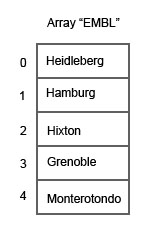
\includegraphics[scale=0.6]{fig/fig2441_arrayScheme.jpg}
\caption{EMBL array}
\label{figEMBLarray}
\end{center}
\end{figure} 
 
Then when you want to retrieve some name from the array, you refer to the address within the array. 
So EMBL[0] will be Heidelberg, EMBL[4] will be Monterotondo, and so on. 
In such a way, files names contained in a folder could be listed and stored, 
or x-y coordinates of free-hand ROI could be stored for further use. 

Here is a macro using the EMBL array example. 

\lstinputlisting[morekeywords={*, newArray}]{code/code20.ijm}

\begin{itemize}
\item Line 3 uses a function that creates a new array (\ilcom{newArray()}),
defined by a parameter for number of array elements (in the example case its 5) and its name \ilcom{EMBL}.
\item From line 4 to 8, each array from position 0 to 4 will be filled with
names (Array starts with 0th element).
\item Line 9 asks the user to input the address (position) within the array.
Then this input address is examined if the address exists within the
\ilcom{EMBL} array in line 10. \ilcom{EMBL.length} returns the number of "boxes"
within the array. If this is satisfied, then line 10 prints out the string in that address.
\end{itemize}

Array could be created and initialized with actual values at the
same time, so line 3 to 8 could be written in a single line like this: 
\begin{lstlisting}[numbers=none]
EMBL = newArray("Heidelberg","Hamburg","Hixton","Grenoble","Monterotondo");
for (i = 0; i < EMBL.length; i++)
    print(EMBL[i]);
\end{lstlisting}
